\section{Systematic risk, the CAPM and factor models}

These entries take the \hyperref[meth:capital-allocation-line]{capital allocation line} to equilibrium and then to factor models. The regression example uses twelve invented months declared in \hyperref[meth:capm-regression]{CAPM regression}; the cost-of-equity example uses inputs published for 1~October~2026. The other examples are invented, and none is evidence about a security or a market.

\begin{qfmechanism}[Systematic and nonsystematic risk: splitting an asset's variance by its covariance with a common return, why diversification removes only the residual part, and the model-dependent claim that only systematic exposure earns a risk premium]\label{mech:systematic-risk-pricing}
\qffield{Statement} Sharpe regards the scatter of an asset's returns $R_i$ around their mean as evidence of its total risk. Part of the scatter is due to the asset's relation with the return $R_g$ of an efficient combination, measured by the slope $B_{ig}$; ``it is this component of the asset's total risk which we term the \emph{systematic} risk'', and the remainder, uncorrelated with $R_g$, ``is the unsystematic component''. The part of an asset's risk due to its correlation with the combination ``cannot be diversified away when the asset is added to the combination'', so prices adjust until $B_{ig}$ is directly related to expected return \citep[\emph{Journal of Finance} 19(3), 1964, pp.~438--440 and Fig.~8]{capital-asset-prices-1964}.

Fama and French give the portfolio reading of beta. The market variance is a value-weighted average of the assets' covariances with the market, so ``$\beta_{iM}$ is proportional to the risk each dollar invested in asset $i$ contributes to the market portfolio'' \citep[\emph{JEP} 18(3), 2004, pp.~28--29 and n.~3]{capm-theory-evidence-2004}. Huberman and Wang describe the covariance in both the CAPM and the APT as ``a measure of risk that investors cannot avoid by diversification'' \citep[FRBNY Staff Report 216, August 2005, sec.~1]{arbitrage-pricing-review-2005}.

\qffield{Notation} With $R_i=a_i+\beta_iR_M+\varepsilon_i$ and $\varepsilon_i$ uncorrelated with $R_M$,
\[ \sigma_i^2=\beta_i^2\sigma_M^2+\sigma_{\varepsilon_i}^2,\qquad \beta_i=\frac{\mathrm{Cov}(R_i,R_M)}{\sigma_M^2}=\rho_{iM}\frac{\sigma_i}{\sigma_M}. \]
The first term is systematic and the second residual (idiosyncratic, nonsystematic). The systematic share of variance is $\rho_{iM}^2$, which a regression reports as $R^2$ (Interpretation).

\qffield{Conditions} \emph{Why residual risk diversifies.} In an equally weighted portfolio of $n$ assets whose residuals are uncorrelated with each other and with bounded variances, residual variance falls like $1/n$ while the systematic part stays (\hyperref[mech:diversification-correlation]{diversification}; \hyperref[mod:factor-risk-model]{factor risk model}, where residual correlation shared by every pair behaves like an omitted factor).

\emph{Why only systematic risk earns a premium.} The claim is a result of a pricing model, not a fact about returns. In the CAPM every investor holds the market portfolio, and an asset's contribution to that portfolio's risk is its covariance with it, so expected excess return is proportional to beta. In the APT, mispriced residual risk can be diversified away and combined into a near-arbitrage (\hyperref[mod:multifactor-apt]{APT}). The conclusion therefore needs investors who are diversified across the relevant assets and a correct specification of the common factors (Interpretation).

Risk that is residual with respect to one market proxy may be systematic with respect to another factor that is priced. Fama and French read the size and value premia as compensation for undiversifiable covariances missed by the market return, a reading that behavioural explanations dispute (pp.~37--40). An investor who is not diversified, such as an owner-manager or a concentrated fund, bears residual risk in fact; the model says only that the market will not pay for it (Interpretation).

\qffield{Practice} Example, original, annual percent: an asset with standard deviation 30 and beta 1.25 against a market with standard deviation 16 has systematic standard deviation $1.25\times16=20$ and residual standard deviation $\sqrt{30^2-20^2}=22.36$; its correlation with the market is $2/3$. Equal-weight portfolios of $n$ such assets with independent residuals have standard deviations of 30.0, 21.21, 20.12 and 20.01 for $n=1$, 10, 100 and 1{,}000, approaching 20.

With the inputs of \hyperref[mod:capm-sml]{CAPM}, a 5.29 percent risk-free rate and a 4.20 percent market premium, the SML gives the asset 10.54 percent. A portfolio on the capital market line with standard deviation 20, the asset's systematic part, has the same 10.54 percent. The capital market line at the asset's own 30 percent would imply 13.165 percent, which is not available for a single asset: its extra 22.36 percent of residual risk earns nothing in the model.

In the twelve-month sample of \hyperref[meth:capm-regression]{CAPM regression}, 81.3 percent of the variation in the stock's excess returns is associated with the market's.

\qffield{Pitfalls} Ranking assets for expected return by total volatility. Concluding that residual risk is irrelevant to an investor who is not diversified, or to an active manager judged against a benchmark. Measuring ``systematic'' risk against a narrow proxy and assuming it is the priced risk. Treating the pricing claim as an empirical finding: the CAPM's version of it fails in the tests reviewed in \hyperref[mod:capm-sml]{CAPM}.

\qffield{See also} \hyperref[mod:return-generating-models]{return-generating models}; \hyperref[mod:capm-sml]{CAPM and the SML}; \hyperref[mod:multifactor-apt]{APT}; \hyperref[mod:factor-risk-model]{factor risk model} (Narang's ``unintended is not the same as uncompensated'').

\end{qfmechanism}

\begin{qfmodel}[Return-generating models: the market (single-index) model and multifactor models as statistical descriptions of returns, how they differ from equilibrium pricing restrictions, and their uses]\label{mod:return-generating-models}
\qffield{Statement} A return-generating model describes how returns vary with common factors; it does not by itself say what expected returns must be. Huberman and Wang write the factor model behind the APT as $r=\mu+\beta f+e$, with $n$ assets, $k$ factors, $E[f]=0$ and $E[e]=0$, so that $E[r]=\mu$. Pricing theory then adds a restriction on $\mu$, exactly $\mu=\imath\lambda_0+\beta\lambda_1$ or approximately \citep[FRBNY Staff Report 216, August 2005, sec.~2, eqs.~(1)--(3)]{arbitrage-pricing-review-2005}.

Ross starts from the same kind of model, $\tilde x_i=E_i+\beta_i\tilde\delta+\tilde\epsilon_i$ \citep[\emph{Journal of Economic Theory} 13, 1976, eq.~(2), p.~342, and eq.~(15), p.~347]{arbitrage-theory-1976}. Sharpe's regression of an asset's return on that of an efficient combination is the single-index form, which he notes ``has been called the diagonal model'' because it makes the covariance matrix easier to handle \citep[\emph{Journal of Finance} 19(3), 1964, pp.~438--439 and n.~23]{capital-asset-prices-1964}.

\qffield{Notation} The \emph{market model} for asset $i$ in period $t$ is
\[ R_{it}=a_i+b_iR_{Mt}+\varepsilon_{it},\qquad E(\varepsilon_{it})=0,\ \mathrm{Cov}(\varepsilon_{it},R_{Mt})=0. \]
In the single-index version the residuals of different assets are also uncorrelated, so $\mathrm{Cov}(R_i,R_j)=b_ib_j\sigma_M^2$ for $i\ne j$. A multifactor return-generating model replaces $b_iR_{Mt}$ by $\sum_kb_{ik}F_{kt}$ (Interpretation).

\qffield{Conditions} \emph{Statistical against pricing.} The market model fits any intercept $a_i$. The Sharpe--Lintner CAPM restricts it: with excess returns the intercept of $R_{it}-R_{ft}=\alpha_i+\beta_{iM}(R_{Mt}-R_{ft})+\varepsilon_{it}$ must be zero \citep[\emph{JEP} 18(3), 2004, p.~32]{capm-theory-evidence-2004}. With a constant risk-free rate the raw-return intercept must then equal $(1-\beta_i)R_f$ (Interpretation). A return-generating model can therefore describe returns well while the pricing restriction fails, and a pricing model can hold with residuals that are correlated across assets.

\emph{Assumptions of the single-index model.} Residual correlation across assets, from industries for example, violates it. Markowitz notes that firms in the same industry tend to do poorly together \citep[\emph{Journal of Finance} 7(1), 1952, p.~89]{s6-markowitz}, and Fama and French name industry effects as a source of common residual variation (p.~31). Parameters estimated over one window need not hold in another, and the index used as ``the market'' is a proxy.

\qffield{Practice} \emph{Uses} (Interpretation, with the sources cited):
\begin{itemize}
\item Estimating beta for the CAPM (\hyperref[meth:required-return-on-equity]{required return on equity}).
\item Building a covariance matrix with few parameters. For 500 assets a full covariance matrix has $500\times501/2=125{,}250$ distinct entries, while the single-index model needs 500 betas, 500 residual variances and one market variance, 1{,}001 in all.
\item Separating market-related from residual returns, as in event studies and performance evaluation. Fama and French list three-factor intercepts used to calibrate price responses to news and to measure managers' information (p.~39).
\item Hedging market exposure with the estimated beta.
\end{itemize}
In the twelve-month example of \hyperref[meth:capm-regression]{CAPM regression}, the market model on raw returns gives $\hat a=0.016$ and $\hat b=1.257$ percent per percent, with $R^2=0.814$.

\qffield{Pitfalls} Reading a market-model intercept as a CAPM alpha. Assuming residuals are independent across stocks of the same industry. Treating a fitted factor structure as evidence for a pricing model; Huberman and Wang stress that any test of the APT is a joint test of the factors and the pricing relation (sec.~6).

\qffield{See also} \hyperref[mech:systematic-risk-pricing]{systematic risk}; \hyperref[mod:capm-sml]{CAPM}; \hyperref[def:factor-model-types]{factor model types}; \hyperref[mod:factor-risk-model]{factor risk model}; \hyperref[meth:simple-regression-estimation]{simple regression}.

\end{qfmodel}

\begin{qfmodel}[The capital asset pricing model: assumptions, beta, the security market line, expected and required returns, the CML against the SML, the Black version, applications and the empirical record]\label{mod:capm-sml}
\qffield{Statement} The CAPM adds two assumptions to Markowitz's model, in which investors are risk averse and care only about the mean and variance of one-period returns. The first is complete agreement on the joint distribution of returns, which is the true one. The second is borrowing and lending at a risk-free rate that is the same for all investors and independent of the amount \citep[\emph{JEP} 18(3), 2004, p.~26]{capm-theory-evidence-2004}. Every investor then holds the same tangency portfolio, which must be the value-weight market portfolio, and the market must lie on the minimum-variance frontier (p.~28). The Sharpe--Lintner relation follows:
\[ E(R_i)=R_f+[E(R_M)-R_f]\,\beta_{iM},\qquad \beta_{iM}=\frac{\mathrm{Cov}(R_i,R_M)}{\sigma^2(R_M)} \]
(pp.~28--29). It holds for portfolios as well as securities, since a portfolio's expected return and beta are the weighted averages of its assets' (p.~31, n.~4). Sharpe states the equilibrium conditions as a common pure rate of interest at which all investors can borrow or lend, and homogeneous expectations, assumptions he calls ``highly restrictive and undoubtedly unrealistic'' \citep[\emph{Journal of Finance} 19(3), 1964, pp.~433--434]{capital-asset-prices-1964}.

Black's version drops risk-free borrowing and lending and allows unrestricted short sales instead. The market is still efficient, and $R_f$ is replaced by the expected return on zero-beta assets, which need only be below the market's (Fama and French, pp.~29--30). With neither a risk-free asset nor short sales, the market portfolio is not typically efficient ``and the CAPM relation between expected return and market beta is lost'' (p.~30).

\qffield{Notation} The \emph{security market line} (SML) plots expected or required return against beta: intercept $R_f$, slope the market premium $E(R_M)-R_f$. The CML plots expected return against \emph{standard deviation} and holds only for efficient portfolios. Every asset and portfolio lies on the SML if the CAPM holds; single assets lie below the CML, because part of their standard deviation is residual (\hyperref[mech:systematic-risk-pricing]{systematic risk}). Interpretation: a security's position against the SML is its alpha, $E(R_i)-[R_f+\beta_i(E(R_M)-R_f)]$.

\qffield{Conditions} Usual further simplifications are a single period, no taxes or transaction costs, divisible assets, price-taking investors and a market portfolio that contains all risky assets (Interpretation). Fama and French note that the market portfolio ``in principle can include not just traded financial assets, but also consumer durables, real estate and human capital'' (p.~25). Roll's critique is that tests use proxies; Fama and French take the pragmatic view that a proxy on the minimum-variance frontier would serve, but no reasonable proxy has been found (pp.~41--42).

\emph{Evidence.} The relation between average return and beta is too flat. For ten beta-sorted US portfolios over 1928--2003, the lowest-beta portfolio was predicted to earn 8.3 percent a year and earned 11.1, and the highest was predicted 16.8 and earned 13.7 (pp.~32--33). Size, earnings--price, debt--equity and book-to-market ratios add explanatory power beyond beta (pp.~35--36). For book-to-market portfolios in 1963--2003 average returns rose from 10.1 to 16.7 percent while beta did not (p.~42, Fig.~3). Their conclusion: ``the CAPM's empirical problems probably invalidate its use in applications'' (p.~44).

\qffield{Practice} Example, original: forward-looking inputs of 1~October~2026, a risk-free rate of 5.29 percent and a market premium of 4.20 percent (\hyperref[meth:required-return-on-equity]{required return on equity}).
\begin{itemize}
\item \emph{Required returns}: 7.81, 9.49, 10.54 and 12.01 percent for betas 0.6, 1.0, 1.25 and 1.6.
\item \emph{A portfolio} 50/30/20 in the 0.6, 1.0 and 1.6 assets has beta 0.92 and required return 9.154 percent, the same weighted average of the assets' required returns.
\item \emph{Security selection}: an analyst who forecasts 11.5 percent for the beta-1.25 stock places it 0.96 percentage points above the SML, a positive alpha relative to the CAPM. It looks underpriced only if both the forecast and the model are right.
\item \emph{Hedging and timing}: beta is the market exposure per unit of capital; selling index futures worth beta times the position removes the market component to the extent that beta is right.
\item \emph{Performance evaluation}: Jensen's alpha is the intercept of the excess-return regression (\hyperref[meth:capm-regression]{CAPM regression}).
\item \emph{CML against SML}: with a market standard deviation of 16 percent, the CML would assign the stock's 30 percent volatility 13.165 percent; the SML assigns its beta 10.54.
\end{itemize}

\begin{center}
% compendium/portfolio-construction-risk/figures/security-market-line.tikz
% Security market line of mod:capm-sml with the forward-looking inputs of 1 October 2026 (risk-free 5.29,
% premium 4.20 percent a year); points rechecked by trading_notes.numerical.asset_pricing_models.asset_pricing_checks.
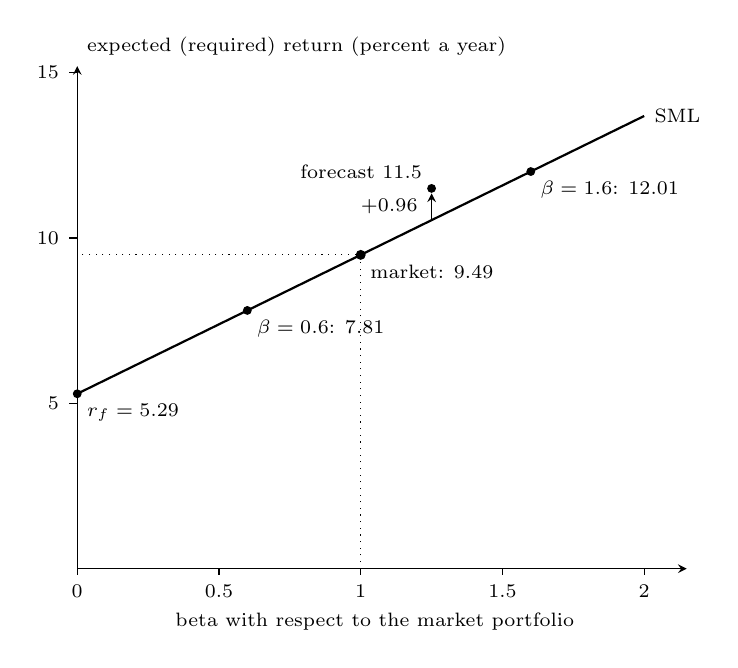
\begin{tikzpicture}[>=stealth, x=3.6cm, y=0.42cm, font=\scriptsize]
  \draw[->] (0,0) -- (2.15,0);
  \node at (1.05,-1.6) {beta with respect to the market portfolio};
  \draw[->] (0,0) -- (0,15.2) node[above right] {expected (required) return (percent a year)};
  \foreach \x in {0,0.5,1,1.5,2} \draw (\x,0) -- (\x,-0.2) node[below] {\x};
  \foreach \y in {5,10,15} \draw (0,\y) -- (-0.03,\y) node[left] {\y};
  \draw[thick] (0,5.29) -- (2,13.69) node[right] {SML};
  \draw[dotted] (1,0) -- (1,9.49) -- (0,9.49);
  % point low
  \fill (0.6,7.81) circle (1.6pt) node[below right] {$\beta=0.6$: 7.81};
  % point market
  \fill (1,9.49) circle (1.8pt) node[below right] {market: 9.49};
  % point high
  \fill (1.6,12.01) circle (1.6pt) node[below right] {$\beta=1.6$: 12.01};
  % point forecast
  \fill (1.25,11.5) circle (1.6pt) node[above left] {forecast 11.5};
  \draw[->, thin] (1.25,10.54) -- (1.25,11.35);
  \node[anchor=east] at (1.235,10.95) {$+0.96$};
  \fill (0,5.29) circle (1.6pt) node[below right] {$r_f=5.29$};
\end{tikzpicture}

\end{center}

\qffield{Pitfalls} Putting standard deviation on the SML's axis or beta on the CML's. Reading a point above the SML as a guaranteed gain. Using the CAPM's required return for a value or small stock without regard to the evidence that it is biased (pp.~43--44). Treating a stock index as the market portfolio of the theory. Fama and French's footnote~7: with a market premium of 8.3 percent a year for 1927--2003 and a standard error of 2.4, the two-standard-error range of 3.5 to 13.1 percent makes most cost-of-equity estimates ``rather meaningless'' (p.~44).

\qffield{See also} \hyperref[meth:capital-allocation-line]{capital allocation line} (CAL and CML); \hyperref[mech:systematic-risk-pricing]{systematic risk}; \hyperref[meth:capm-regression]{CAPM regression}; \hyperref[meth:required-return-on-equity]{required return on equity}; \hyperref[mod:multifactor-apt]{APT and multifactor models}; \hyperref[meth:relative-performance-evaluation]{relative performance evaluation}.

\end{qfmodel}

\begin{qfmethod}[Estimating CAPM alpha and beta by regression: aligned excess returns, closed forms and an independent least-squares check, units, fit and uncertainty, raw-return against excess-return regressions, and why a fitted alpha is not skill]\label{meth:capm-regression}
\qffield{Statement} The Sharpe--Lintner CAPM implies a time-series test. When an asset's excess return is regressed on the market's excess return, ``Jensen's alpha'', the intercept, ``is zero for each asset'' \citep[\emph{JEP} 18(3), 2004, p.~32]{capm-theory-evidence-2004}:
\[ R_{it}-R_{ft}=\alpha_i+\beta_{iM}(R_{Mt}-R_{ft})+\varepsilon_{it}. \] Least squares estimates the coefficients as in \hyperref[meth:simple-regression-estimation]{simple regression}: $\hat\beta=S_{xy}/S_{xx}$ and $\hat\alpha=\bar y-\hat\beta\bar x$, with $y$ the asset's and $x$ the market's excess return. Huberman and Wang give the same estimators for a factor regression \citep[FRBNY Staff Report 216, August 2005, sec.~7, eqs.~(14)--(17)]{arbitrage-pricing-review-2005}.

\qffield{Data} Invented and declared: twelve months of total returns in percent, typed by hand, for a stock S, a market index M and a one-month Treasury bill whose rate rises through the year. Each row is the same calendar month for all three, and the bill rate is the return on a bill held over that month. S was built as $r_f+0.1+1.25(R_M-r_f)$ plus hand-chosen residuals, rounded; the estimates do not use this.

\begin{center}\small
\begin{tabular}{@{}lrrrrrrrrrrrr@{}}
\toprule
Month & 1 & 2 & 3 & 4 & 5 & 6 & 7 & 8 & 9 & 10 & 11 & 12 \\
\midrule
$R_S$ & 3.6 & $-3.3$ & 2.6 & 2.8 & $-3.6$ & 0.5 & 6.6 & $-0.2$ & $-0.8$ & $-3.0$ & 3.7 & 1.6 \\
$R_M$ & 2.1 & $-1.4$ & 3.0 & 0.8 & $-2.6$ & 1.9 & 4.2 & $-0.7$ & 1.1 & $-3.3$ & 2.5 & 0.6 \\
$R_f$ & 0.30 & 0.31 & 0.32 & 0.33 & 0.35 & 0.36 & 0.38 & 0.39 & 0.40 & 0.41 & 0.42 & 0.42 \\
\bottomrule
\end{tabular}
\end{center}

\qffield{Practice} \emph{Estimates.} $\hat\beta=1.2548$ and $\hat\alpha=0.1108$ percent a month. The closed forms, a matrix least-squares solution and a regression package agree, and $\hat\beta$ equals the sample covariance of the excess returns divided by the market's sample variance with either denominator. The residual standard deviation is 1.447 percent a month and $R^2=0.813$. The standard errors are 0.190 for $\hat\beta$ and 0.422 for $\hat\alpha$, with 10 degrees of freedom. The 95 percent intervals are 0.83 to 1.68 for beta and $-0.83$ to $1.05$ for alpha ($t=0.26$).

\emph{Interpretation.} Beta is unit-free: in this sample a month in which the market's excess return was one percentage point higher came with a stock excess return about 1.25 points higher on average. Alpha is in percent a month; twelve times it is 1.33 percent a year, with an interval of $-9.95$ to $12.61$. $R^2$ is the share of the sample variance of the stock's excess return associated with the market: 81 percent systematic and 19 percent residual (\hyperref[mech:systematic-risk-pricing]{systematic risk}).

\emph{Raw against excess returns.} Regressing raw $R_S$ on raw $R_M$, the market model, gives $\hat a=0.0158$ and $\hat b=1.2574$. The intercepts differ by $-0.0949$, of which $(1-\hat\beta)\bar R_f=-0.0932$ comes from the risk-free rate's place in the model and $-0.0017$ from its variation over the year. With a constant risk-free rate the two slopes coincide and $\hat a=\hat\alpha+(1-\hat\beta)R_f$ exactly. A raw intercept is thus not Jensen's alpha: for a high-beta asset it is lower by about $(\beta-1)R_f$, and the gap grows with the level of rates (Interpretation).

\qffield{Conditions} \emph{Alignment.} The three series must cover the same periods, use total returns in the same currency, and use a bill rate for the same holding period, known at its start. The market index is a proxy, and its choice changes beta. The standard errors assume the conditions in \hyperref[meth:regression-diagnostics-anova]{regression diagnostics}: errors that are independent and of constant variance. Return data often violate both, and nonsynchronous trading biases betas estimated from short intervals (Interpretation).

\emph{Uncertainty.} Twelve observations are far too few. Fama and French call individual betas ``imprecise'' (p.~31) and note that large standard errors of betas and of the premium make cost-of-equity estimates ``rather meaningless'' (p.~44, n.~7). Betas also change over time; Harris measures them concurrently for this reason (\hyperref[meth:relative-performance-evaluation]{relative performance evaluation}).

\emph{Alpha is not skill.} A fitted alpha measures the average excess return not associated with the market proxy in that sample, given the model. It can reflect luck: here the interval spans more than 22 percentage points a year. It can also reflect the model's failure: funds tilted to low-beta, small or value stocks ``will tend to produce positive abnormal returns'' against the Sharpe--Lintner CAPM ``even when the fund managers have no special talent for picking winners'' (p.~44). Testing for skill needs a credible benchmark and the inference in \hyperref[meth:skill-luck-significance-tests]{skill against luck}.

\qffield{Pitfalls} Regressing raw returns and calling the intercept alpha. Mixing a stock's total return with a price-only index. Using an annual bill yield in a monthly regression. Annualising a monthly alpha without its uncertainty. Reporting beta without its interval or estimation window.

\qffield{See also} \hyperref[mod:return-generating-models]{return-generating models}; \hyperref[mod:capm-sml]{CAPM}; \hyperref[meth:required-return-on-equity]{required return on equity}; \hyperref[meth:simple-regression-estimation]{simple regression}; \hyperref[meth:regression-diagnostics-anova]{regression diagnostics}.

\end{qfmethod}

\begin{qfmethod}[Estimating a required return on equity with the CAPM: a forward-looking risk-free rate, equity premium and beta, the market model's role, sensitivity, and the difference from a historical average or fitted return]\label{meth:required-return-on-equity}
\qffield{Statement} The textbook prescription that Fama and French describe is ``to estimate a stock's market beta and combine it with the risk-free interest rate and the average market risk premium to produce an estimate of the cost of equity'' \citep[\emph{JEP} 18(3), 2004, p.~43]{capm-theory-evidence-2004}:
\[ k_e=r_f+\beta_i\,\mathrm{ERP}. \]
The required return is the expected return investors demand for bearing the equity's risk. It is a forward-looking rate for discounting the firm's expected cash flows, and ``the cost of capital is forward looking, so if the premiums are sample specific they are irrelevant'' (p.~40).

\qffield{Data} Inputs for 1~October~2026, in US dollars, nominal, percent a year:
\begin{itemize}
\item \emph{Equity risk premium}: Damodaran's implied premium on 1~October~2026 was 4.20 percent on his base method (trailing twelve-month cash flows with adjusted payout). His four other variants gave 3.70, 5.67, 3.61 and 3.30 percent \citep[home page, ``Equity Risk Premiums'', read 2026-10-18]{implied-equity-premium-2026}.
\item \emph{Risk-free rate}: he computed those premia against a US Treasury rate of 5.29 percent, and noted that netting out a 0.22 percent default spread would give 5.07 percent (same page). The Treasury's 10-year par yield was 5.29 percent on 30~September~2026 \citep[2026 file, retrieved 2026-10-18]{ust-par-yield-curve}.
\item \emph{Beta}: 1.15, an assumption of the example, standing for a forward-looking beta that an analyst would justify from a longer estimation window, comparable firms or an adjustment; it is not the twelve-month estimate.
\end{itemize}

\qffield{Practice} $k_e=5.29+1.15\times4.20=10.12$ percent. Across the published premia, 3.30 to 5.67 percent, it ranges from 9.09 to 11.81 percent. Holding the premium at 4.20, the twelve-month beta interval of 0.83 to 1.68 (\hyperref[meth:capm-regression]{CAPM regression}) gives 8.78 to 12.34 percent.

\emph{A historical premium instead.} The 1928--2025 arithmetic average excess return of US stocks over 10-year Treasury bonds was 7.03 percent (\hyperref[def:asset-class-characteristics]{asset classes}). Added with the same beta to the current 10-year yield, it gives $5.29+1.15\times7.03=13.38$ percent; the geometric-average premium of 5.48 percent gives 11.60. This is a standard CAPM estimate, not a mismatch: the premium was measured over 10-year bonds and is added to the current 10-year yield.

The two estimates differ in their assumption about the premium. The implied premium is read from current prices and expected cash flows; the historical premium assumes that the premium realised in the past is a good estimate of the premium expected now. Damodaran presents the choice as a point of view: to keep a valuation market neutral, use the current implied premium; ``if you believe that numbers revert back to historical averages, use the historical premium'' \citep[``Project Emails/Information'', sec.~V.b ``Risk Premiums'', read 2026-10-18]{corporate-finance-project-notes}.

The historical estimate is also imprecise. Treating the years as independent, the arithmetic premium has a standard error of about 2.10 percentage points. A band of two standard errors (2.83 to 11.24 percent) moves $k_e$ from 8.54 to 18.21 percent, and the choice between arithmetic and geometric averages alone moves it by 1.8 points (Interpretation). Fama and French report a standard error of 2.4 points for the 1927--2003 market premium over Treasury bills (p.~44, n.~7).

\emph{The market model's role.} The regression of the stock's returns on the market's supplies beta. Its intercept is not part of the required return, and the fitted return $\hat a+\hat bR_M$ reproduces the sample's average return. In the twelve-month example that average is $0.875\times12=10.50$ percent a year. It is a description of one past year, whose closeness to 10.12 is coincidence, not an estimate of what investors require (Interpretation).

\qffield{Conditions} The rate, premium and beta must refer to the same currency, horizon and market, and the premium must be defined against the kind of risk-free rate that is added back (Interpretation). Damodaran's project notes take the 10-year government bond rate in the currency of the analysis as the riskless rate (sec.~V.a), and advise against estimating a historical premium for a non-US company from its own market's history (sec.~V.b).

\emph{For a historical premium}, the matching rate is the current yield on the security over which the excess returns were measured, here the 10-year Treasury bond. Adding a bond-based premium to a bill rate, or the reverse, mixes benchmarks. The approach also assumes that past realised premia inform the expected premium. Its estimation error, and its sensitivity to the sample period, the averaging method and the country, are part of the estimate (Interpretation).

\emph{For an implied premium}, the matching rate is the one used to solve for it. Damodaran's 4.20 percent was computed against 5.29 percent. Pairing it with another rate, or with his spread-adjusted 5.07 percent without also adding the 0.22 percent spread to the premium, changes $k_e$ mechanically with no change in view; that is a different error from choosing a historical premium. A long-term government yield suits long-lived equity cash flows better than a bill rate, and a nominal rate makes $k_e$ nominal, to be applied to nominal cash flows (Interpretation).

The estimate inherits the CAPM's empirical problems. Fama and French find CAPM costs of equity ``too high (relative to historical average returns)'' for high-beta stocks and too low for low-beta and value stocks (pp.~43--44). Multifactor alternatives, such as the three-factor model offered by practitioners for the cost of equity (p.~39), or the APT used in utility rate cases \citep[FRBNY Staff Report 216, August 2005, sec.~9]{arbitrage-pricing-review-2005}, give different answers depending on the factors chosen.

\qffield{Pitfalls} Treating the result as precise to a basis point. Adding a premium to a different risk-free rate from the one it was measured or solved against: a bond-based premium to a bill rate, or an implied premium to a rate other than its own. Reporting a historical premium without its period, averaging method and standard error, or as if the past premium must recur. Using the trailing sample average return as the required return. Using a raw twelve-month beta for a firm whose business or leverage has changed.

\qffield{See also} \hyperref[mod:capm-sml]{CAPM and the SML}; \hyperref[meth:capm-regression]{CAPM regression}; \hyperref[def:asset-class-characteristics]{asset classes} (historical against expected returns).

\end{qfmethod}

\begin{qfmodel}[Multifactor pricing and arbitrage pricing theory: factor exposures, factor risk premia, residual risk, expected returns from sensitivities, exact arbitrage among well-diversified portfolios and residual-risk-bearing approximations]\label{mod:multifactor-apt}
\qffield{Statement} Ross's heuristic for the APT starts from a factor model in which residuals are independent enough for the law of large numbers to hold \citep[\emph{Journal of Economic Theory} 13, 1976, pp.~342--343]{arbitrage-theory-1976}:
\begin{itemize}
\item form an \emph{arbitrage portfolio} that uses no wealth and is well diversified;
\item for large $n$ its residual return becomes negligible;
\item choose it to have no systematic risk, so that its return is certain;
\item to rule out arbitrarily large positions, that certain return must be zero.
\end{itemize}
Expected returns are then spanned by a constant and the factor sensitivities, $E_i=\rho+\lambda\beta_i$, where $\rho$ is the riskless rate or, without a riskless asset, the zero-beta return. The argument suggests the relation holds ``in all but the most profound sort of disequilibria'', and ``the market portfolio plays no special role'' (p.~343). With $k$ factors, an asset's premium is ``the $\beta$-weighted sum of the factor risk premiums'' $E^k-\rho$, where $E^k$ is the return on a portfolio with unit sensitivity to factor $k$ and none to the others (p.~353, eq.~(24)).

\qffield{Notation} In the notation of Huberman and Wang, $r=\mu+\beta f+e$, and exact arbitrage pricing is $\mu=\imath\lambda_0+\beta\lambda_1$. $\beta$ holds the \emph{factor exposures} (loadings or sensitivities), $\lambda_1$ the \emph{factor risk premia}, the expected return per unit of exposure, and $e$ the \emph{residual} return. The APT in general asserts only the approximate form $(\mu-X\lambda)'Z^{-1}(\mu-X\lambda)\le a$ for a constant $a$, with $X=(\imath,\beta)$; exact pricing is the case $a=0$ \citep[FRBNY Staff Report 216, August 2005, sec.~2, eqs.~(1)--(3)]{arbitrage-pricing-review-2005}.

\qffield{Conditions} \emph{Exact and approximate.} Huberman formalises arbitrage as a sequence of zero-cost portfolios whose expected income grows without bound while its variance vanishes. If residual covariances are diagonal and bounded, no arbitrage implies the approximate bound, and the exact relation holds in the limit for well-diversified portfolios, whose residual variance is zero (sec.~4). Ross proves that the sum of squared pricing deviations stays bounded as the number of assets grows (Theorem~I, eq.~(18), p.~347). For any finite set of assets, individual mispricings are therefore allowed.

His rough calibration for 1962--1971 put the average absolute discrepancy below 0.084 percent, ``about 1\% of the market return'' (pp.~353--354).

\emph{Further assumptions.} The bound needs agents whose relative risk aversion is uniformly bounded. Ross's counterexample, a single agent with constant absolute risk aversion, shows that pricing need not converge to the APT without such a condition (secs.~I--II, pp.~344--347). The APT does not need mean--variance preferences, normal returns or the market portfolio. It needs less agreement than the CAPM: investors must share expectations and the factor sensitivities, but may disagree about the factors' distributions (p.~355).

The theory does not name the factors, so ``any test of the APT is a joint test that the factors are correctly identified and that the linear pricing relation holds'' (Huberman and Wang, sec.~8). It concerns static portfolios, so using it to evaluate dynamically managed portfolios is ``contradictory to the no-arbitrage spirit of the model'' (abstract; sec.~9). Multifactor pricing can also come from equilibrium: in Merton's ICAPM investors care about covariances with state variables, which requires betas on further factors as well as the market \citep[\emph{JEP} 18(3), 2004, pp.~37--38]{capm-theory-evidence-2004}.

\qffield{Practice} \emph{Expected return from sensitivities}, original, annual percent: with $\lambda_0=4$ and premia of 3 for factor 1 and 1.5 for factor 2, a stock with sensitivities $(1.2,-0.4)$ should return $4+3.6-0.6=7.0$ percent, a premium of 3.0 over $\lambda_0$. The negative sensitivity lowers the required return: the stock pays off when factor 2 is bad for other holdings.

\emph{An arbitrage}, original. Well-diversified portfolios A, B and C have sensitivities $(1.0,0.5)$, $(0.5,-0.5)$ and $(1.5,1.0)$ and expected returns 7.75, 4.75 and 10.00 percent; solving the three pricing equations recovers $\lambda_0=4$, $\lambda=(3,1.5)$. A fourth well-diversified portfolio D with sensitivities $(0.8,0.2)$ should earn $4+2.4+0.3=6.70$ percent but is priced to earn 7.50. Weights $(1.0,0.2,-0.2)$ in A, B and C have D's sensitivities, sum to one and earn 6.70.

Buying 1{,}000{,}000 of D and selling 1{,}000{,}000 of that replica costs nothing and has no factor exposure. If D and the replica have no residual risk, it earns a certain 8{,}000 a year, an exact arbitrage that the APT rules out; prices must move until D yields 6.70.

\emph{Residual risk.} If D is instead one stock with a residual standard deviation of 25 percent, the same trade has expected profit 8{,}000 and standard deviation 250{,}000: it is a bet, not an arbitrage. Spread over $n$ such stocks with independent residuals and the same mispricing, the residual standard deviation of the position falls to $25/\sqrt n$ percent, 2.5 at $n=100$ and 0.5 at $n=2{,}500$, small but never zero. This is why the APT restricts prices only approximately for individual assets (Interpretation). Factor sensitivities are themselves estimated, so in practice even a well-diversified version carries model risk.

\emph{Empirical premia.} Fama and French's three-factor model, $E(R_{it})-R_{ft}=\beta_{iM}[E(R_{Mt})-R_{ft}]+\beta_{is}E(\mathrm{SMB}_t)+\beta_{ih}E(\mathrm{HML}_t)$, is described as in the spirit of both the ICAPM and the APT. Over 1927--2003 the average premia were 8.3, 3.6 and 5.0 percent a year, with standard deviations of 21.0, 14.6 and 14.2: ``high volatility implies substantial uncertainty about the true expected premiums'' (pp.~38--39).

\qffield{Pitfalls} Confusing a factor sensitivity with a factor premium, or a factor's realised return with its expected premium. Calling a trade with residual risk an arbitrage. Concluding from any set of factors that fit average returns that the APT is confirmed: a mean--variance efficient portfolio always exists and can serve as a ``factor'' (Huberman and Wang, sec.~6).

\qffield{See also} \hyperref[mod:return-generating-models]{return-generating models}; \hyperref[def:factor-model-types]{factor model types}; \hyperref[mod:capm-sml]{CAPM}; \hyperref[mech:systematic-risk-pricing]{systematic risk}; \hyperref[mod:factor-risk-model]{factor risk model}.

\end{qfmodel}

\begin{qfdefinition}[Macroeconomic, fundamental and statistical factor models: inputs, estimation, outputs and interpretation, their uses in risk, attribution, pricing and construction, the value of several risk dimensions, and their limitations]\label{def:factor-model-types}
\qffield{Statement} Connor divides multifactor models of returns into three types \citep[\emph{Financial Analysts Journal}, May--June 1995, pp.~42--43 and Table~1]{factor-model-types-1995}:
\begin{itemize}
\item \emph{Macroeconomic} models use observable economic time series, such as inflation, industrial production, the excess return on long-term government bonds and the premium of low-grade over high-grade corporate bonds, as measures of the pervasive shocks. Each security's factor betas are estimated by time-series regression, which ``requires a long and stable history of returns''.
\item \emph{Fundamental} models use observed company attributes, such as size, dividend yield, book-to-market and industry, as the factor betas. The factors are the realised returns of mimicking portfolios, estimated each period by cross-sectional regression: the dividend-yield factor is ``the realized return per extra unit of dividend yield, holding other attributes constant''.
\item \emph{Statistical} models derive both factors and betas from returns alone by factor analysis or principal components. Their factors are ``essentially unlabeled statistical artifacts'' that can be linearly recombined.
\end{itemize}
Without estimation error and with unlimited data the three are ``rotations of one another'' and can all hold at once (p.~43).

Huberman and Wang describe three ways of identifying factors. The first is an algorithmic analysis of the covariance matrix. The second is a researcher's judgement guided by it, as in the size and book-to-market factors of Fama and French. The third is pure judgement, as in Chen, Roll and Ross's financial and macroeconomic variables. Only the first two respect the factor structure, and the third is ``more in the spirit of Merton's (1973) intertemporal CAPM than in the spirit of the APT'' \citep[FRBNY Staff Report 216, August 2005, sec.~8]{arbitrage-pricing-review-2005}.

\qffield{Data} Connor's comparison covers 779 large-capitalisation US stocks, January 1985 to December 1993, with explanatory power measured as one minus average specific variance over average total variance (pp.~44--45, Tables~2--5):
\begin{itemize}
\item five statistical factors explain 39.0 percent, the first alone 29.0;
\item five macroeconomic factors explain 10.9 percent, needing both the default and the term-structure factors;
\item the fundamental model of 55 industry dummies and 12 risk indices explains 42.6 percent, the industries alone 16.3;
\item the macroeconomic model adds nothing once the fundamental model is included.
\end{itemize}
He adds that by theoretical consistency and intuitive appeal the macroeconomic model ``is probably the strongest'' of the three (p.~46).

\qffield{Conditions} \emph{Comparison} (Interpretation, from the sources cited and \hyperref[mod:factor-risk-model]{factor risk model}):
\begin{itemize}
\item \emph{Macroeconomic.} The factors are economic surprises, which must be measured as unexpected changes, and the exposures are estimated. The model is interpretable, linked to theory and useful for macro scenarios. Its limitations are low explanatory power, error in measuring surprises, and betas that need long, stable histories.
\item \emph{Fundamental.} The exposures are observed and current, and the factor returns are estimated. The model responds immediately to changes in a firm and its explanatory power is high. It depends on vendor definitions and many inputs, and its industry factors carry much of the fit.
\item \emph{Statistical.} The model needs returns data only and fits the sample best. Its factors are unlabeled, defined only up to sign and rotation, and unstable across samples.
\end{itemize}

All three are return-generating descriptions. Pricing requires the further restriction of \hyperref[mod:multifactor-apt]{APT} or an equilibrium model, and evidence that a factor explains covariance does not show that it carries a premium.

\qffield{Practice} \emph{Uses and outputs.} Common uses (Interpretation):
\begin{itemize}
\item Risk decomposition into factor and specific parts, with contributions by factor.
\item Return attribution.
\item Control or hedging of unintended exposures in construction (\hyperref[mod:factor-risk-model]{factor risk model}).
\item Expected returns and costs of capital. Huberman and Wang report macroeconomic and Fama--French factor models proposed for utility rate cases in New York, where the commission used the CAPM instead (sec.~9).
\item Performance evaluation with factor alphas, and asset allocation with fewer parameters, since $k$ factor portfolios span the efficient frontier when the factor model holds (sec.~9).
\end{itemize}

Example, original, monthly percent, a fundamental model with market, size and value factors. A portfolio's exposures are $(1.0,-0.3,0.6)$ against its benchmark's $(1.0,0,0.1)$, so its active exposures are $(0,-0.3,0.5)$. In a month with factor returns 2.0, $-0.8$ and 1.2, the factors explain $0+0.24+0.60=0.84$ percentage points of active return. If the realised active return was 1.10, 0.26 is specific to the holdings.

With factor covariance matrix rows $(16,2,-1)$, $(2,9,0.5)$ and $(-1,0.5,6.25)$ and a specific variance of 4.0, the portfolio's factor variance is $x^\top Fx=16.48$ and its total 20.48, so factors account for 80.5 percent. The contributions $x_k(Fx)_k$ are 14.80 from the market, 0.12 from size and 1.56 from value. The output says the portfolio's risk is mostly market risk and its size tilt barely matters for risk, though it added 0.24 to this month's return.

\emph{Several risk dimensions.} Two portfolios with the same market beta of 1.0 but inflation sensitivities of $+0.5$ and $-0.5$ look identical to the CAPM. A month with a market factor return of $-2$ and an inflation factor return of $+1$ moves them $-1.5$ and $-2.5$ percent. Modelling several dimensions shows such differences. It allows a risk budget or hedge per source, and it matches investors who care about covariances with state variables such as labour income or inflation, as in the ICAPM \citep[\emph{JEP} 18(3), 2004, pp.~37--38]{capm-theory-evidence-2004}.

\qffield{Pitfalls} Naming a statistical factor after the fact and treating the name as a property of the method. Reading a factor's explanatory power as evidence that it is priced. Adding factors until a sample is explained: Huberman and Wang note that ``the number of factors, as well as the methods of factor construction, is exploding'' (sec.~8). Comparing exposures from different models as if their factors were the same.

\qffield{See also} \hyperref[mod:factor-risk-model]{factor risk model} (the covariance decomposition and economic against statistical factors); \hyperref[mod:multifactor-apt]{APT and multifactor models}; \hyperref[mod:return-generating-models]{return-generating models}; \hyperref[meth:portfolio-covariance-estimation]{covariance estimation}.

\end{qfdefinition}
